\section{Managing Python Applications}
One key capability of the \srgui is to start, stop and monitor \py applications running on the \jx.
Currently one \py application is managing all the \gls{ptp} Deamons and one is running the \gls{sensorpipeline}.
Each has their own tab in the \srgui as shown in Figure \ref{fig:gui_map}.

\begin{figure}[H]
    \centering
    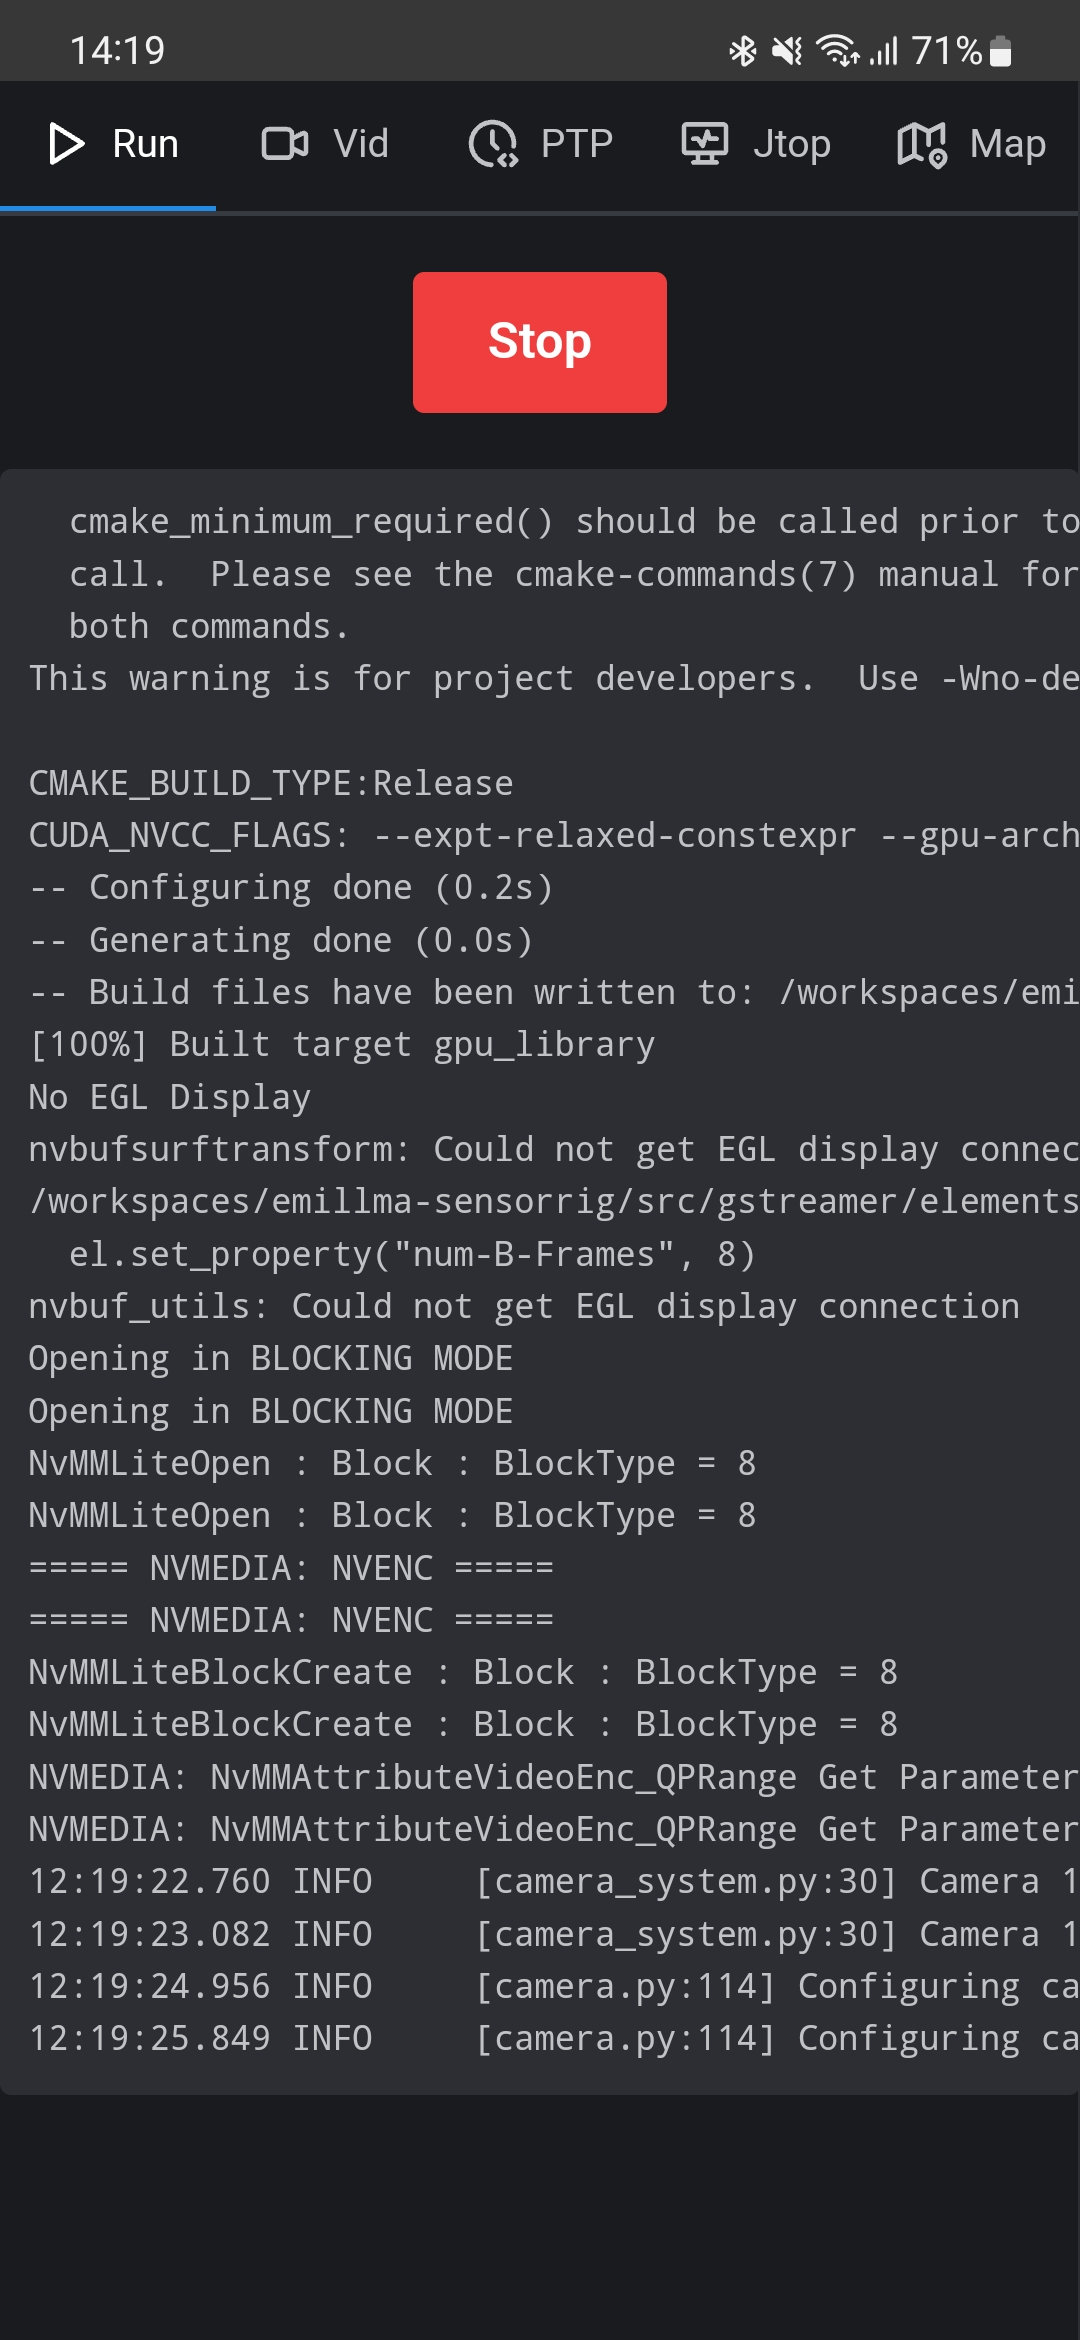
\includegraphics[width=.48\textwidth]{figures/gui/run.jpg}
    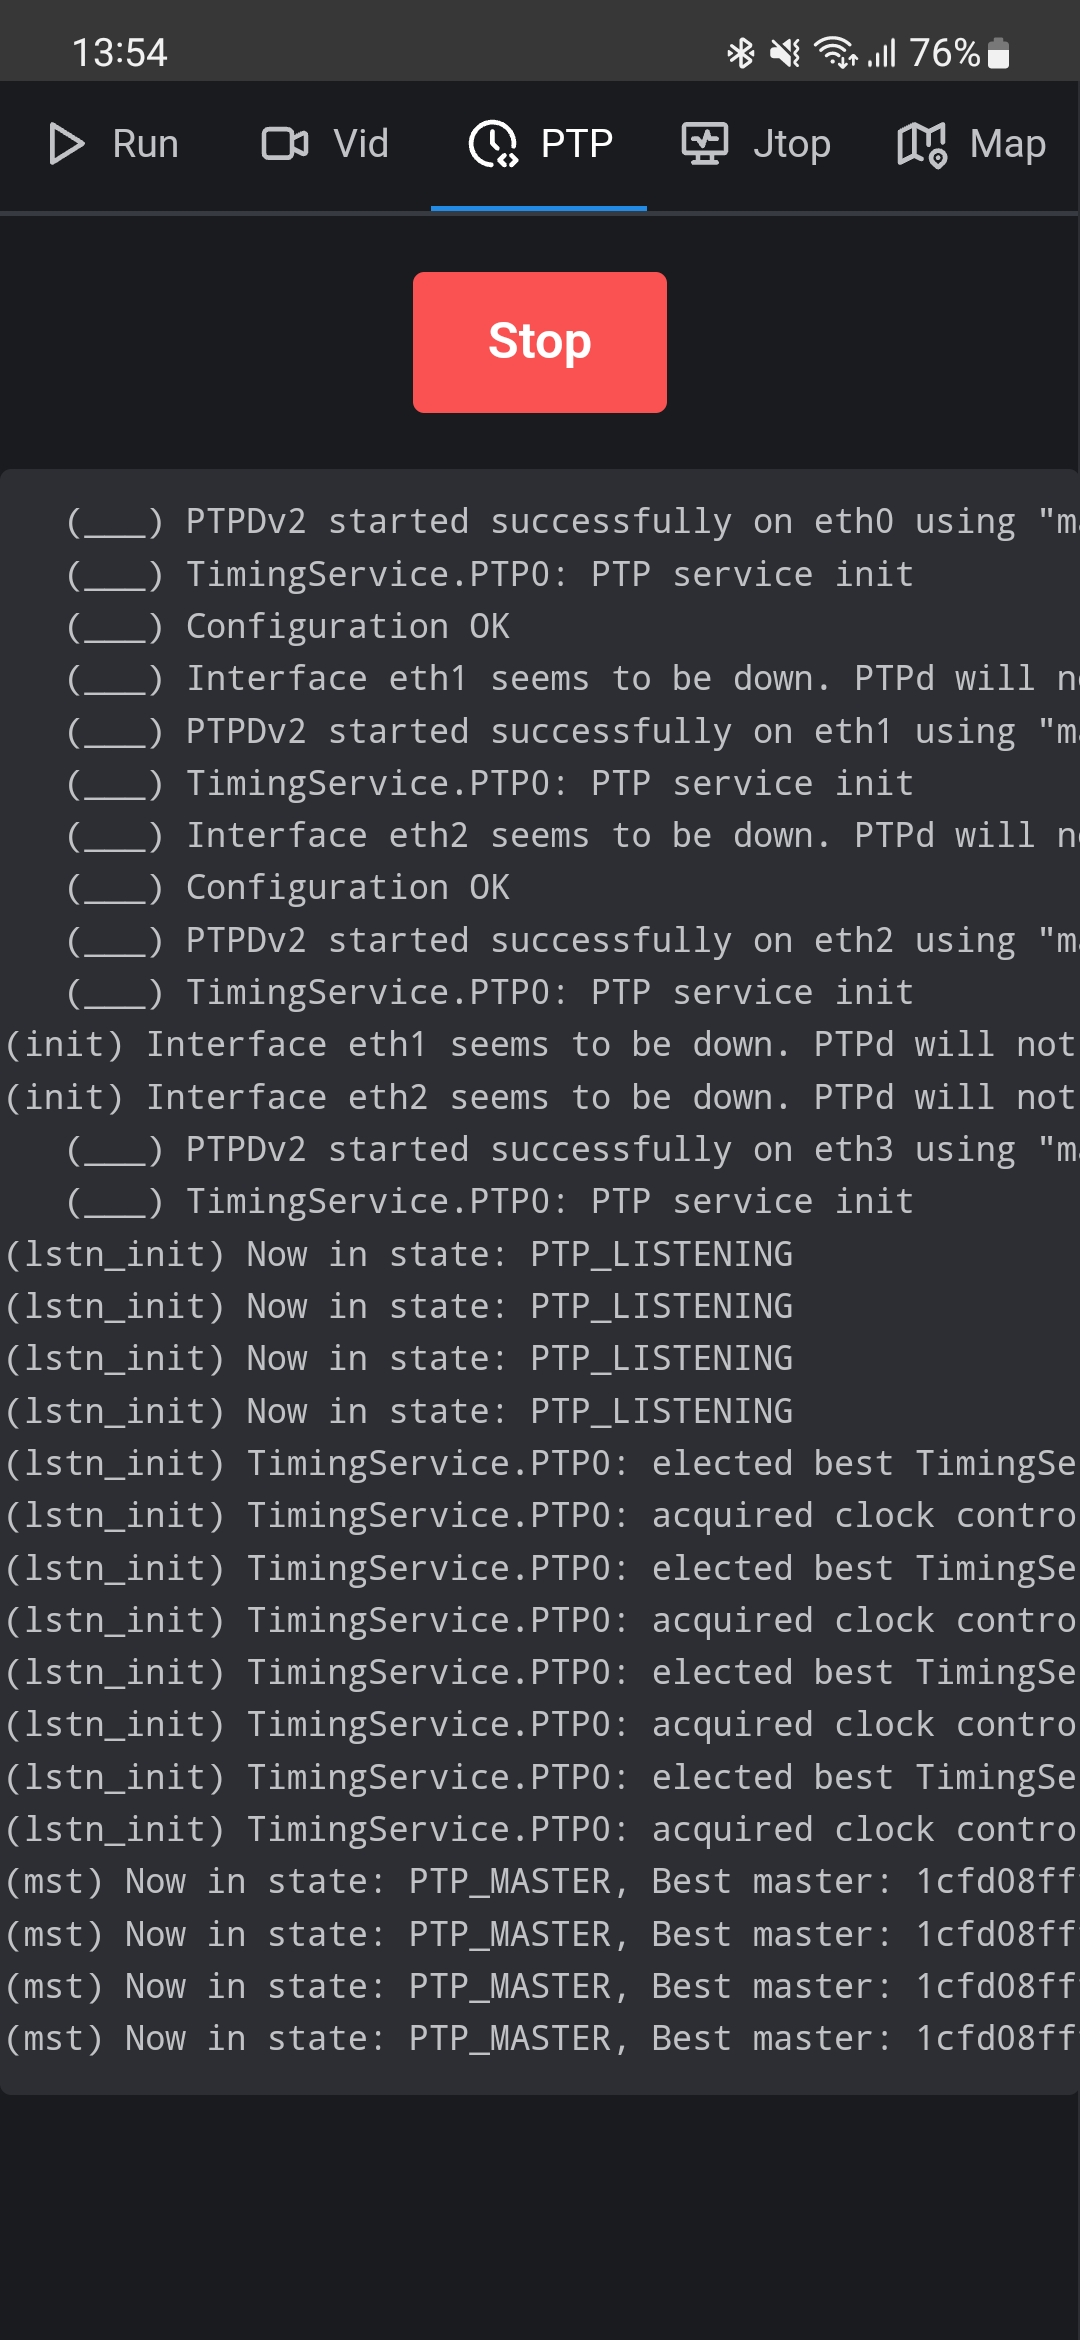
\includegraphics[width=.48\textwidth]{figures/gui/ptp.jpg}
    \caption{Screenshot of Run and PTP tab of \srgui used to start, stop and monitor the two \py applications, with applications running.}
    \label{fig:gui_map}
\end{figure}

Every time a \gls{ptp} Deamon is stopped and started the \cams use quite a long time to synchronize their time, it is thus better to keep the \gls{ptp} Deamons running separately.

In the current setup the